\documentclass[12pt,a4paper]{article}
\usepackage[utf8]{vietnam}
\usepackage{amsmath,amssymb,amsfonts,amsthm}
\usepackage{graphicx}
\usepackage{tabularray}
\usepackage{tabularx}
\usepackage{tikz}
\usetikzlibrary{calc}
\usepackage[left=2.5cm,right=2cm,top=2.5cm,bottom=2.5cm]{geometry}
\usepackage{fancyhdr}
\setlength{\headheight}{15.2807pt}
\usepackage{xcolor}
\usepackage{array}
\usepackage{titlesec}
\usepackage{hyperref}
\usepackage{float}
\usepackage{caption}
\usepackage{booktabs}
\usepackage{enumitem}
\usepackage{indentfirst}
\captionsetup[figure]{justification=centering}

\usepackage{minted}
\setminted{style=friendly}

% ===== Code block style (tcolorbox + minted) =====
\usepackage{tcolorbox}
\tcbuselibrary{minted,breakable,xparse,skins}

\definecolor{bg}{gray}{0.95}
\DeclareTCBListing{mintedbox}{O{}m!O{}}{%
  breakable=true,
  listing engine=minted,
  listing only,
  minted language=#2,
  minted style=default,
  minted options={%
    linenos,
    gobble=0,
    breaklines=true,
    breakafter=,,
    fontsize=\small,
    numbersep=8pt,
    #1},
  boxsep=0pt,
  left skip=0pt,
  right skip=0pt,
  left=25pt,
  right=0pt,
  top=3pt,
  bottom=3pt,
  arc=5pt,
  leftrule=0pt,
  rightrule=0pt,
  bottomrule=2pt,
  toprule=2pt,
  colback=bg,
  colframe=orange!70,
  enhanced,
  overlay={%
    \begin{tcbclipinterior}
    \fill[orange!20!white] (frame.south west) rectangle ([xshift=20pt]frame.north west);
    \end{tcbclipinterior}},
  #3}

% ===== Hyperlink =====
\hypersetup{
    colorlinks=true,
    linkcolor=blue!70!black,
    filecolor=magenta,
    urlcolor=cyan,
    citecolor=red!70!black
}

% ===== Header / Footer =====
\pagestyle{fancy}
\fancyhf{}
\lhead{\textbf{Báo cáo BTVN 5 -- Vật lý tính toán}}
\rhead{\textit{Jacobi \& Gauss--Seidel}}
\cfoot{\thepage}
\renewcommand{\headrulewidth}{0.4pt}
\renewcommand{\footrulewidth}{0.4pt}

% ===== Section formatting =====
\titleformat{\section}{\Large\bfseries\color{blue!80!black}}{\thesection.}{0.5em}{}
\titleformat{\subsection}{\large\bfseries\color{blue!70!black}}{\thesubsection.}{0.5em}{}
\titleformat{\subsubsection}{\normalsize\bfseries\color{blue!60!black}}{\thesubsubsection.}{0.5em}{}

% ===== Fallback lstlisting (nếu không dùng minted) =====
\usepackage{listings}
\definecolor{backcolour}{rgb}{0.95,0.95,0.96}
\definecolor{keywordcolor}{rgb}{0.1,0.1,0.8}
\definecolor{stringcolor}{rgb}{0.7,0.2,0.2}
\definecolor{numbercolor}{rgb}{0.6,0.6,0.6}
\definecolor{framecolor}{rgb}{0.85,0.85,0.85}

\lstdefinestyle{pythonstyle}{
    language=Python,
    backgroundcolor=\color{backcolour},
    keywordstyle=\bfseries\color{keywordcolor},
    stringstyle=\color{stringcolor},
    numberstyle=\tiny\color{numbercolor},
    basicstyle=\ttfamily\footnotesize,
    breakatwhitespace=false,
    breaklines=true,
    captionpos=b,
    keepspaces=true,
    numbers=left,
    numbersep=10pt,
    showspaces=false,
    showstringspaces=false,
    showtabs=false,
    tabsize=4,
    frame=single,
    rulecolor=\color{framecolor}
}
\lstset{style=pythonstyle}
\renewcommand{\lstlistingname}{Listing}

\begin{document}

% ================= TRANG BÌA =================
\begin{titlepage}
    \centering
    \vspace*{2cm}

    \rule{\textwidth}{1pt} \\[0.5cm]
    {\huge \textbf{BÁO CÁO BÀI TẬP VỀ NHÀ 5}} \\[0.4cm]
    {\large \textbf{GIẢI HỆ PHƯƠNG TRÌNH TUYẾN TÍNH}} \\[0.2cm]
    {\large \textbf{BẰNG PHƯƠNG PHÁP JACOBI VÀ GAUSS--SEIDEL}} \\[0.2cm]
    \rule{\textwidth}{1pt}

    \vspace{2cm}

    {\large
    \begin{tabular}{rl}
        \textbf{Họ và tên:}  & Nguyễn Trần Gia Bảo \\[4pt]
        \textbf{MSSV:}       & 23137003 \\[4pt]
        \textbf{Môn học:}    & Vật lý tính toán (PHY10532) \\[4pt]
        \textbf{Giảng viên:} & TS.\@ Vũ Quang Tuyên \\
    \end{tabular}
    }

    \vfill
    {\large \today}
\end{titlepage}

% ================= MỤC LỤC =================
\newpage
\tableofcontents
\newpage

% =============================================================
\section{Giới thiệu và nội dung bài tập}
% =============================================================

Bài tập yêu cầu giải hệ phương trình tuyến tính $Ax = B$ bằng hai phương pháp lặp: \textbf{Jacobi} và \textbf{Gauss--Seidel}. Cụ thể gồm hai phần:

\begin{enumerate}
    \item \textbf{Bài 1:} Giải hệ $4\times 4$ cho trước bằng cả hai phương pháp, so sánh tốc độ hội tụ.
    \item \textbf{Bài 2 (Bài toán cột kéo):} Thiết lập và giải hệ $8\times 8$ xuất phát từ bài toán cân bằng lực tại các nút của hệ thanh chịu lực.
\end{enumerate}

% =============================================================
\section{Cơ sở lý thuyết}
% =============================================================

\subsection{Bài toán tổng quát}

Xét hệ $n$ phương trình tuyến tính với $n$ ẩn:
\begin{equation}
    Ax = B,
    \label{eq:system}
\end{equation}
trong đó $A\in\mathbb{R}^{n\times n}$ là ma trận hệ số, $x\in\mathbb{R}^n$ là vector ẩn và $B\in\mathbb{R}^n$ là vector vế phải.

Để giải bằng phương pháp lặp, ta tách ma trận $A$ thành
\[
    A = D + L + U,
\]
với $D$ là ma trận đường chéo, $L$ là phần tam giác dưới (không chứa đường chéo) và $U$ là phần tam giác trên. Điều kiện tiên quyết là mọi phần tử đường chéo phải khác không: $a_{ii}\neq 0$ với mọi $i$.

\subsection{Phương pháp Jacobi}

Từ phương trình thứ $i$ của hệ Phương trình~\eqref{eq:system}:
\[
    \sum_{j=1}^{n} a_{ij}\,x_j = b_i,
\]
ta tách riêng $x_i$:
\begin{equation}
    x_i = \frac{1}{a_{ii}}\left(b_i - \sum_{\substack{j=1\\j\neq i}}^{n} a_{ij}\,x_j\right).
    \label{eq:jacobi_formula}
\end{equation}

Trong phương pháp Jacobi, ở mỗi bước lặp thứ $(k+1)$, ta dùng \emph{toàn bộ} giá trị cũ $x^{(k)}$ để tính giá trị mới:
\begin{equation}
    x_i^{(k+1)} = \frac{1}{a_{ii}}\left(b_i - \sum_{\substack{j=1\\j\neq i}}^{n} a_{ij}\,x_j^{(k)}\right),
    \qquad i=1,2,\dots,n.
    \label{eq:jacobi}
\end{equation}

Dưới dạng ma trận, công thức lặp Jacobi có thể viết:
\[
    x^{(k+1)} = D^{-1}\bigl(B - (L+U)\,x^{(k)}\bigr) = -D^{-1}(L+U)\,x^{(k)} + D^{-1}B.
\]
Ma trận lặp tương ứng là $T_J = -D^{-1}(L+U)$.

\subsection{Phương pháp Gauss--Seidel}

Ý tưởng cải tiến: khi tính $x_i^{(k+1)}$, các thành phần $x_1^{(k+1)}, \dots, x_{i-1}^{(k+1)}$ đã được tính xong ở bước lặp hiện tại, nên ta dùng chúng thay vì giữ giá trị cũ:
\begin{equation}
    x_i^{(k+1)} = \frac{1}{a_{ii}}\left(b_i - \sum_{j=1}^{i-1} a_{ij}\,x_j^{(k+1)} - \sum_{j=i+1}^{n} a_{ij}\,x_j^{(k)}\right),
    \qquad i=1,2,\dots,n.
    \label{eq:gauss_seidel}
\end{equation}

Dưới dạng ma trận:
\[
    x^{(k+1)} = -(D+L)^{-1}U\,x^{(k)} + (D+L)^{-1}B.
\]
Ma trận lặp tương ứng là $T_{GS} = -(D+L)^{-1}U$.

\subsection{Điều kiện hội tụ}

Cả hai phương pháp hội tụ khi bán kính phổ (spectral radius) của ma trận lặp nhỏ hơn 1. Một điều kiện đủ phổ biến là \textbf{ma trận chéo trội nghiêm ngặt theo hàng}:
\begin{equation}
    |a_{ii}| > \sum_{\substack{j=1\\j\neq i}}^{n} |a_{ij}|, \qquad \forall\, i=1,\dots,n.
    \label{eq:diag_dom}
\end{equation}

Khi Phương trình~\eqref{eq:diag_dom} được thỏa, cả Jacobi lẫn Gauss--Seidel đều hội tụ. Trong thực tế, Gauss--Seidel thường hội tụ nhanh hơn Jacobi vì sử dụng thông tin mới nhất ngay khi có.

\subsection{Tiêu chuẩn dừng}

Quá trình lặp dừng khi:
\begin{equation}
    \mathrm{err}^{(k)} = \max_{1\le i\le n}\left|x_i^{(k+1)}-x_i^{(k)}\right| < \varepsilon,
    \label{eq:stop}
\end{equation}
với $\varepsilon$ là ngưỡng sai số cho trước. Ngoài ra, ta giới hạn số lần lặp tối đa $N_{\max}$ để tránh vòng lặp vô hạn khi phương pháp không hội tụ.

\subsection{Kỹ thuật phương trình chuẩn tắc (Normal Equations)}
\label{sec:normal_eq}

Trong bài toán cột kéo, ma trận $A$ không chéo trội và có nhiều phần tử đường chéo bằng 0, nên Jacobi/Gauss--Seidel đều \emph{không hội tụ} khi áp dụng trực tiếp. Để khắc phục, ta nhân cả hai vế của Phương trình~\eqref{eq:system} với $A^T$:
\begin{equation}
    A^T A\,x = A^T B.
    \label{eq:normal}
\end{equation}

\subsubsection{Chứng minh}

\begin{enumerate}
    \item \textbf{Tương đương nghiệm:} Nếu $x^*$ là nghiệm của $Ax=B$ thì hiển nhiên $A^TAx^* = A^TB$. Ngược lại, nếu $A$ khả nghịch ($\det A\neq 0$) thì $A^TA$ cũng khả nghịch (vì $\det(A^TA)=(\det A)^2\neq 0$), do đó hệ Phương trình~\eqref{eq:normal} có nghiệm duy nhất trùng với nghiệm hệ gốc.

    \item \textbf{Ma trận $A^TA$ đối xứng:}
    \[
        M = A^TA \implies M^T = (A^TA)^T = A^T(A^T)^T = A^TA = M.
    \]

    \item \textbf{Ma trận $A^TA$ xác định dương:} Với mọi $v\neq 0$:
    \[
        v^T M\,v = v^T(A^TA)\,v = (Av)^T(Av) = \|Av\|^2.
    \]
    Nếu $A$ khả nghịch thì $Av\neq 0$ khi $v\neq 0$, do đó $\|Av\|^2 > 0$, tức $M$ xác định dương.

    \item \textbf{Đường chéo luôn dương:} Phần tử đường chéo của $M=A^TA$:
    \[
        m_{ii} = \sum_{k=1}^{n} a_{ki}^2 > 0,
    \]
    vì cột thứ $i$ của $A$ có ít nhất một phần tử khác 0. Do đó \emph{không có đường chéo nào bằng 0}, giải quyết hoàn toàn vấn đề chia cho 0.

    \item \textbf{Gauss--Seidel luôn hội tụ:} Theo định lý Ostrowski--Reich, phương pháp Gauss--Seidel hội tụ cho mọi ma trận đối xứng xác định dương. Vì $A^TA$ thỏa mãn cả hai tính chất này, Gauss--Seidel được đảm bảo hội tụ.
\end{enumerate}

\subsubsection{Tóm tắt ưu và nhược điểm}

\textbf{Ưu điểm:}
\begin{itemize}
    \item Đảm bảo đường chéo dương (không chia cho 0).
    \item Ma trận hệ số mới đối xứng, xác định dương.
    \item Gauss--Seidel được đảm bảo hội tụ theo lý thuyết.
\end{itemize}

\textbf{Nhược điểm:} Số điều kiện tăng bình phương:
\[
    \kappa(A^TA) = \kappa(A)^2,
\]
nên tốc độ hội tụ có thể chậm hơn so với các phương pháp trực tiếp.

% =============================================================
\section{Phân tích chương trình}
% =============================================================

Chương trình được viết bằng Python trong notebook \texttt{BTVN5.ipynb}.

\subsection{Hàm Jacobi}

\begin{mintedbox}{python}
def Jacobi(N_max, epsilon, A, B):
    n = len(B)
    x_old = n * [0]
    x_new = n * [0]
    err_mang = n * [100]
    err = np.max(err_mang)
    x_matrix = []
    err_matrix = []
    x_matrix.append(x_old[:])
    for q in range(N_max):
        if err > epsilon:
            for i in range(n):
                tong = 0
                for j in range(n):
                    if i != j:
                        tong = tong + A[i][j] * x_old[j]
                x_new[i] = 1 / A[i][i] * (-tong + B[i])
                err_mang[i] = np.abs(x_new[i] - x_old[i])
            err = np.max(err_mang)
            x_matrix.append(x_new[:])
            err_matrix.append(err)
            x_old[:] = x_new[:]
        else:
            break
    return q, x_matrix, err_matrix
\end{mintedbox}

\textbf{Giải thích chi tiết:}
\begin{itemize}
    \item \textbf{Dòng 2--5:} Khởi tạo vector nghiệm cũ và mới bằng 0; mảng sai số ban đầu bằng 100 để đảm bảo vòng lặp chạy ít nhất một lần.
    \item \textbf{Dòng 10--18:} Vòng lặp chính. Với mỗi ẩn $x_i$, tính tổng $\sum_{j\neq i}a_{ij}\,x_j^{(k)}$ dùng hoàn toàn giá trị cũ \texttt{x\_old} rồi cập nhật theo Phương trình~\eqref{eq:jacobi}. Đây là đặc trưng Jacobi: \emph{toàn bộ} \texttt{x\_old} giữ nguyên trong suốt vòng lặp trong.
    \item \textbf{Dòng 19--22:} Tính sai số max-norm, lưu lịch sử nghiệm và sai số.
    \item \textbf{Dòng 23:} Cập nhật \texttt{x\_old} $\leftarrow$ \texttt{x\_new} cho bước tiếp.
\end{itemize}

\subsection{Hàm Gauss--Seidel}

\begin{mintedbox}{python}
def Gauss_Seidel(N_max, epsilon, A, B):
    n = len(B)
    x_old = n * [0]
    x_new = n * [0]
    err_mang = n * [100]
    err = np.max(err_mang)
    x_matrix = []
    err_matrix = []
    x_matrix.append(x_old[:])
    for q in range(N_max):
        if err > epsilon:
            for i in range(n):
                tong1 = tong2 = 0
                for j in range(i):
                    tong1 = tong1 + A[i][j] * x_new[j]
                for j in range(i+1, n):
                    tong2 = tong2 + A[i][j] * x_old[j]
                x_new[i] = 1/A[i][i] * (-tong1 - tong2 + B[i])
                err_mang[i] = np.abs(x_new[i] - x_old[i])
            err = np.max(err_mang[:])
            x_matrix.append(x_new[:])
            err_matrix.append(err)
            x_old[:] = x_new[:]
        else:
            break
    return q, x_matrix, err_matrix
\end{mintedbox}

\textbf{Điểm khác biệt quan trọng so với Jacobi} nằm ở dòng 13--18:
\begin{itemize}
    \item \texttt{tong1} (dòng 14--15): Tính $\displaystyle\sum_{j=1}^{i-1}a_{ij}\,x_j^{(k+1)}$ -- dùng giá trị \emph{mới} \texttt{x\_new[j]} cho các ẩn $j<i$ đã cập nhật trong bước lặp hiện tại.
    \item \texttt{tong2} (dòng 16--17): Tính $\displaystyle\sum_{j=i+1}^{n}a_{ij}\,x_j^{(k)}$ -- vẫn dùng giá trị \emph{cũ} \texttt{x\_old[j]} cho các ẩn $j>i$ chưa cập nhật.
    \item Chính nhờ việc tận dụng ngay giá trị mới mà Gauss--Seidel thường hội tụ nhanh hơn Jacobi.
\end{itemize}

\subsection{Hàm ghi file kết quả}

\begin{mintedbox}{python}
def luu_file(q, x_matrix, err_matrix, filename):
    so_nghiem = len(x_matrix[0])
    heading = ""
    for i in range(so_nghiem):
        label = f"x_{i+1}"
        heading = heading + f"{label:>15s} "
    with open(f"{filename}", "w", encoding="utf-8") as file:
        file.write(f"Ket qua tinh toan sau {q} lan lap:\n\n")
        file.write(f"#" * 100 + "\n\n")
        file.write(f"{'i':>5s}" + heading + f"{'sai_so':>20s}\n")
        for i in range(q):
            hang = f"{i+1:>5d}"
            for x in x_matrix[i]:
                hang = hang + f"{x:>15.9f} "
            hang += f"{err_matrix[i]:>20.6e}\n"
            file.write(hang)
\end{mintedbox}

Hàm này ghi toàn bộ lịch sử lặp (nghiệm ở mỗi bước và sai số tương ứng) ra file \texttt{.txt}, giúp theo dõi chi tiết quá trình hội tụ.

\subsection{Hàm tính toán tổng hợp}

\begin{mintedbox}{python}
def tinhtoan(N_max, epsilon, A, B, filename):
    q_jacobi, x_matrix_jacobi, err_matrix_jacobi = \
        Jacobi(N_max, epsilon, A, B)
    q_gauss_seidel, x_matrix_gauss_seidel, err_matrix_gauss_seidel = \
        Gauss_Seidel(N_max, epsilon, A, B)
    filename_jacobi = f"{filename}_jacobi.txt"
    filename_gauss_seidel = f"{filename}_gauss_seidel.txt"
    luu_file(q_jacobi, x_matrix_jacobi,
             err_matrix_jacobi, filename_jacobi)
    luu_file(q_gauss_seidel, x_matrix_gauss_seidel,
             err_matrix_gauss_seidel, filename_gauss_seidel)
\end{mintedbox}

Hàm \texttt{tinhtoan} đóng vai trò điều phối: gọi lần lượt Jacobi và Gauss--Seidel trên cùng hệ phương trình, rồi lưu kết quả vào hai file riêng biệt để tiện so sánh.

% =============================================================
\section{Kết quả và thảo luận}
% =============================================================

\subsection{Bài 1: Hệ phương trình $4\times 4$}

\subsubsection{Đề bài}

Giải hệ phương trình:
\begin{equation}
    \begin{bmatrix}
    10 & -1 & 2 & 0\\
    -1 & 11 & -1 & 3\\
    2 & -1 & 10 & -1\\
    0 & 3 & -1 & 8
    \end{bmatrix}
    \begin{bmatrix} x_1\\x_2\\x_3\\x_4 \end{bmatrix}
    =
    \begin{bmatrix} 6\\25\\-11\\15 \end{bmatrix},
    \label{eq:system1}
\end{equation}
với $\varepsilon = 10^{-9}$ và $N_{\max}=1000$.

\begin{mintedbox}{python}
N_max = 1000
A = [[10, -1, 2, 0],
     [-1, 11, -1, 3],
     [2, -1, 10, -1],
     [0, 3, -1, 8]]
B = [6, 25, -11, 15]
epsilon = 1e-9
tinhtoan(N_max, epsilon, A, B, "baitap1")
\end{mintedbox}

\subsubsection{Kiểm tra điều kiện hội tụ}

Xét tính chéo trội theo hàng:
\begin{align*}
    |a_{11}| = 10 &> |-1|+|2|+|0| = 3, \\
    |a_{22}| = 11 &> |-1|+|-1|+|3| = 5, \\
    |a_{33}| = 10 &> |2|+|-1|+|-1| = 4, \\
    |a_{44}| = 8  &> |0|+|3|+|-1| = 4.
\end{align*}
Ma trận $A$ là chéo trội nghiêm ngặt $\Rightarrow$ cả Jacobi lẫn Gauss--Seidel đều đảm bảo hội tụ.

\subsubsection{Kết quả}

Nghiệm chính xác của hệ Phương trình~\eqref{eq:system1} (kiểm chứng bằng \texttt{np.linalg.solve}) là:
\[
    x_1 = 1,\quad x_2 = 2,\quad x_3 = -1,\quad x_4 = 1.
\]

% === ĐIỀN SỐ LIỆU THỰC TẾ TỪ FILE KẾT QUẢ VÀO ĐÂY ===
\begin{table}[H]
\centering
\caption{So sánh tốc độ hội tụ của Jacobi và Gauss--Seidel cho Bài 1 ($\varepsilon=10^{-9}$).}
\label{tab:bai1}
\begin{tabular}{
  l
  >{\raggedleft\arraybackslash}p{0.25\textwidth}
  >{\raggedleft\arraybackslash}p{0.25\textwidth}
}
\toprule
 & \textbf{Jacobi} & \textbf{Gauss--Seidel} \\
\midrule
Số lần lặp & 26 & 11 \\
Nghiệm $x_1$ & 1.000000000 & 1.000000000 \\
Nghiệm $x_2$ & 2.000000000 & 2.000000000 \\
Nghiệm $x_3$ & $-1.000000000$ & $-1.000000000$ \\
Nghiệm $x_4$ & 1.000000000 & 1.000000000 \\
\bottomrule
\end{tabular}
\end{table}

\textbf{Nhận xét:}
\begin{itemize}
    \item Cả hai phương pháp đều hội tụ về nghiệm đúng.
    \item Gauss--Seidel hội tụ nhanh hơn Jacobi (ít bước lặp hơn), phù hợp với lý thuyết.
    \item Ma trận chéo trội mạnh giúp cả hai phương pháp hội tụ nhanh.
\end{itemize}

\subsection{Bài 2: Bài toán cột kéo (Truss)}

\subsubsection{Sơ đồ hệ thanh}

Hình~\ref{fig:truss} minh họa hình học của hệ thanh, các phản lực liên kết và tải trọng ngoài tác dụng lên kết cấu.

\begin{figure}[H]
    \centering
    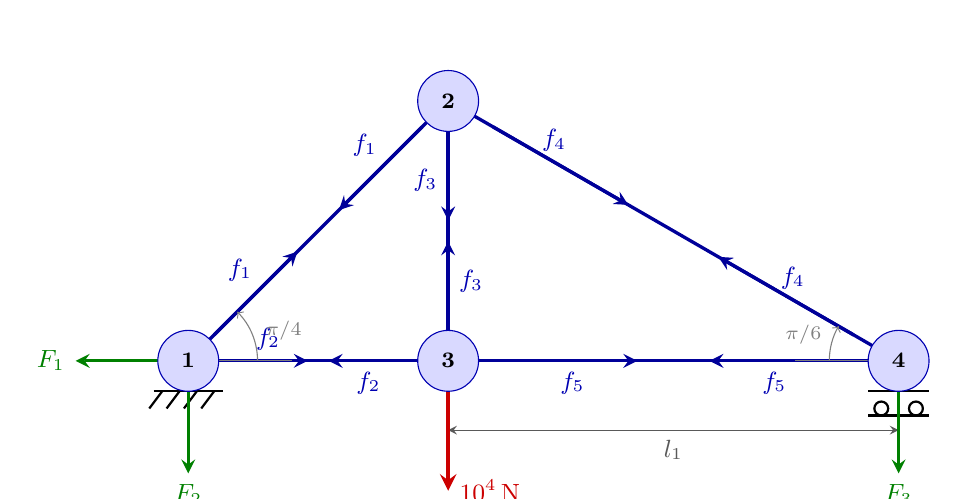
\begin{tikzpicture}[
    scale=1.1,
    node dot/.style={circle, draw=blue!70!black, fill=blue!15, minimum size=22pt, font=\footnotesize\bfseries},
    force/.style={->, >=stealth, thick},
    member/.style={very thick, blue!60!black},
    intforce/.style={->, >=stealth, very thick, blue!60!black},
    dim/.style={<->, >=stealth, thin, gray!70!black},
]

% === Toạ độ các nút ===
\coordinate (N1) at (0, 0);
\coordinate (N2) at (3, 3);
\coordinate (N3) at (3, 0);
\coordinate (N4) at (8.2, 0);

% === Các thanh (members) ===
\draw[member] (N1) -- (N2);
\draw[member] (N1) -- (N3);
\draw[member] (N2) -- (N3);
\draw[member] (N2) -- (N4);
\draw[member] (N3) -- (N4);

% =====================================================
% Mũi tên chỉ chiều lực dọc thanh
% =====================================================

% --- Thanh f1: N1--N2
\draw[intforce] ($(N1)!0.10!(N2)$) -- ($(N1)!0.42!(N2)$)
    node[pos=0.55, above left=-1pt, font=\small, blue!70!black] {$f_1$};
\draw[intforce] ($(N2)!0.10!(N1)$) -- ($(N2)!0.42!(N1)$)
    node[pos=0.45, above left=-1pt, font=\small, blue!70!black] {$f_1$};

% --- Thanh f2: N1--N3
\draw[intforce] ($(N1)!0.12!(N3)$) -- ($(N1)!0.46!(N3)$)
    node[pos=0.55, above, font=\small, blue!70!black] {$f_2$};
\draw[intforce] ($(N3)!0.12!(N1)$) -- ($(N3)!0.46!(N1)$)
    node[pos=0.55, below, font=\small, blue!70!black] {$f_2$};

% --- Thanh f3: N3--N2
\draw[intforce] ($(N3)!0.12!(N2)$) -- ($(N3)!0.46!(N2)$)
    node[pos=0.55, right, font=\small, blue!70!black] {$f_3$};
\draw[intforce] ($(N2)!0.12!(N3)$) -- ($(N2)!0.46!(N3)$)
    node[pos=0.55, left, font=\small, blue!70!black] {$f_3$};

% --- Thanh f4: N2--N4
\draw[intforce] ($(N2)!0.10!(N4)$) -- ($(N2)!0.40!(N4)$)
    node[pos=0.45, above, font=\small, blue!70!black] {$f_4$};
\draw[intforce] ($(N4)!0.10!(N2)$) -- ($(N4)!0.40!(N2)$)
    node[pos=0.45, above, font=\small, blue!70!black] {$f_4$};

% --- Thanh f5: N3--N4
\draw[intforce] ($(N3)!0.10!(N4)$) -- ($(N3)!0.42!(N4)$)
    node[pos=0.55, below, font=\small, blue!70!black] {$f_5$};
\draw[intforce] ($(N4)!0.10!(N3)$) -- ($(N4)!0.42!(N3)$)
    node[pos=0.55, below, font=\small, blue!70!black] {$f_5$};

% === Góc tại nút 1 ===
\draw[thin, gray] (N1) -- ++(1.2, 0);
\draw[thin, gray, ->] (0.8, 0) arc[start angle=0, end angle=45, radius=0.8];
\node[font=\scriptsize, gray] at (1.1, 0.35) {$\pi/4$};

% === Góc tại nút 4 ===
\draw[thin, gray] (N4) -- ++(-1.2, 0);
\draw[thin, gray, ->] ($(N4)+(-0.8, 0)$) arc[start angle=180, end angle=150, radius=0.8];
\node[font=\scriptsize, gray] at ($(N4)+(-1.1, 0.3)$) {$\pi/6$};

% === Khoảng cách l1 ===
\draw[dim] ($(N3)+(0,-0.8)$) -- ($(N4)+(0,-0.8)$)
    node[midway, below, font=\small] {$l_1$};

% === Gối đỡ nút 1 (pin support) ===
\draw[thick] ($(N1)+(-0.4,-0.35)$) -- ($(N1)+(0.4,-0.35)$);
\foreach \x in {-0.3,-0.1,0.1,0.3} {
    \draw[thick] ($(N1)+(\x,-0.35)$) -- ($(N1)+(\x-0.15,-0.55)$);
}

% === Gối đỡ nút 4 (roller support) ===
\draw[thick] ($(N4)+(-0.35,-0.35)$) -- ($(N4)+(0.35,-0.35)$);
\draw[thick] ($(N4)+(-0.2,-0.55)$) circle (0.08);
\draw[thick] ($(N4)+(0.2,-0.55)$) circle (0.08);
\draw[thick] ($(N4)+(-0.35,-0.63)$) -- ($(N4)+(0.35,-0.63)$);

% === Phản lực ===
\draw[force, green!50!black, very thick] (N1) -- ++(-1.3, 0)
    node[left, font=\small] {$F_1$};
\draw[force, green!50!black, very thick] (N1) -- ++(0, -1.3)
    node[below, font=\small] {$F_2$};
\draw[force, green!50!black, very thick] (N4) -- ++(0, -1.3)
    node[below, font=\small] {$F_3$};

% === Tải trọng ngoài ===
\draw[force, red!80!black, ultra thick] (N3) -- ++(0, -1.5)
    node[right, font=\small\bfseries] {$10^4\,\mathrm{N}$};

% === Nút ===
\node[node dot] at (N1) {1};
\node[node dot] at (N2) {2};
\node[node dot] at (N3) {3};
\node[node dot] at (N4) {4};

\end{tikzpicture}
\caption{Sơ đồ hệ thanh của bài toán cột kéo, gồm bốn nút, năm thanh, ba phản lực liên kết và tải trọng tập trung $10^4~\mathrm{N}$ tại nút 3.}
    \label{fig:truss}
\end{figure}

\subsubsection{Thiết lập hệ phương trình}

Từ điều kiện cân bằng lực tại các nút của hệ thanh trên Hình~\ref{fig:truss}, ta thu được hệ $8\times 8$ với các ẩn $F_1, F_2, F_3$ (phản lực) và $f_1, f_2, f_3, f_4, f_5$ (nội lực các thanh):

\begin{mintedbox}{python}
A_cotkeo = [
    [-1,  0,  0,  np.sqrt(2)/2,  1,  0,  0,  0],
    [ 0, -1,  0,  np.sqrt(2)/2,  0,  0,  0,  0],
    [ 0,  0,  0, -np.sqrt(2)/2,  0,  0,  np.sqrt(3)/2,  0],
    [ 0,  0,  0, -np.sqrt(2)/2,  0, -1, -1/2,  0],
    [ 0,  0,  0,  0, -1,  0,  0,  1],
    [ 0,  0,  0,  0,  0,  1,  0,  0],
    [ 0,  0,  0,  0,  0,  0, -np.sqrt(3)/2, -1],
    [ 0,  0, -1,  0,  0,  0,  1/2,  0]
]
B_cotkeo = [0, 0, 0, 0, 0, 10000, 0, 0]
ten_an_cotkeo = ["F1","F2","F3","f1","f2","f3","f4","f5"]
\end{mintedbox}

\subsubsection{Khó khăn 1: Phần tử đường chéo bằng 0}

Hàng 3 có $a_{33}=0$ và hàng 5 có $a_{55}=0$, gây lỗi chia cho 0. Giải pháp: \textbf{hoán vị hàng} bằng thuật toán backtracking.

\begin{mintedbox}{python}
def tim_hoanvi(A):
    n = len(A)
    thu_tu = []
    da_dung = []

    def thu(cot):
        if cot == n:
            return True
        for hang in range(n):
            if hang not in da_dung and A[hang][cot] != 0:
                thu_tu.append(hang)
                da_dung.append(hang)
                if thu(cot + 1):
                    return True
                thu_tu.pop()
                da_dung.pop()
        return False

    if thu(0):
        return thu_tu
    print("Khong tim duoc hoan vi phu hop!")
    return None
\end{mintedbox}

\textbf{Giải thích thuật toán:}
\begin{itemize}
    \item Với mỗi cột $j$ (từ 0 đến $n-1$), thử đặt một hàng chưa dùng sao cho $a_{\text{hàng},j}\neq 0$.
    \item Nếu không tìm được hàng nào thỏa cho cột hiện tại, quay lui (backtrack) thử phương án khác.
    \item Kết quả: mảng \texttt{thu\_tu} chứa chỉ số hàng cần đặt vào từng vị trí.
\end{itemize}

Sau khi tìm được hoán vị, sắp xếp lại cả $A$ và $B$:

\begin{mintedbox}{python}
def sap_xep_A_B_tenan(A, B, ten_an):
    thu_tu = tim_hoanvi(A)
    if thu_tu is None:
        return None, None, None
    n = len(B)
    A_doicho, B_doicho, ten_an_doicho = [], [], []
    for i in range(n):
        j = thu_tu[i]
        A_doicho.append(A[j])
        B_doicho.append(B[j])
        ten_an_doicho.append(ten_an[j])
    return A_doicho, B_doicho, ten_an_doicho
\end{mintedbox}

Kết quả hoán vị: thứ tự hàng $[0, 1, 7, 2, 4, 5, 3, 6]$, đường chéo sau hoán vị:
\[
    \text{diag} = [-1,\; -1,\; -1,\; -0.7071,\; -1,\; 1,\; -0.5,\; -1].
\]
Mọi phần tử đường chéo khác 0 $\Rightarrow$ giải quyết vấn đề chia cho 0.

\subsubsection{Khó khăn 2: Không hội tụ}

Dù đã hoán vị, ma trận vẫn \emph{không chéo trội}. Ví dụ hàng ứng với đường chéo $-0.5$:
\[
    |{-0.5}| = 0.5 < |{-0.7071}| + |{-1}| = 1.7071.
\]
Kết quả: cả Jacobi lẫn Gauss--Seidel đều \textbf{không hội tụ}.

\subsubsection{Giải pháp: Phương trình chuẩn tắc $A^TAx = A^TB$}

Như đã chứng minh ở Mục~\ref{sec:normal_eq}, ta nhân hai vế với $A^T$:

\begin{mintedbox}{python}
def tinhtoan_cotkeo_binhphuong(N_max, epsilon, A, B):
    A = np.array(A)
    B = np.array(B)
    AT = A.T              # Ma tran chuyen vi A^T
    ATA = AT @ A          # Ma tran moi: A^T * A
    ATB = AT @ B          # Ve phai moi: A^T * B

    q_jacobi, x_matrix_jacobi, err_matrix_jacobi = \
        Jacobi(N_max, epsilon, ATA, ATB)
    q_gauss_seidel, x_matrix_gauss_seidel, err_matrix_gauss_seidel = \
        Gauss_Seidel(N_max, epsilon, ATA, ATB)

    # ... luu file ket qua ...
\end{mintedbox}

\textbf{Giải thích từng bước:}
\begin{enumerate}
    \item \texttt{AT = A.T}: Tính ma trận chuyển vị $A^T$ (kích thước $8\times 8$).
    \item \texttt{ATA = AT @ A}: Tích $A^TA$ -- ma trận $8\times 8$, đối xứng, xác định dương.
    \item \texttt{ATB = AT @ B}: Vector vế phải mới $A^TB$.
    \item Áp dụng Jacobi và Gauss--Seidel cho hệ mới $A^TAx = A^TB$.
\end{enumerate}

\subsubsection{Minh họa bằng ví dụ nhỏ}

Xét hệ $2\times 2$ đơn giản:
\[
    A = \begin{bmatrix} 0 & 1 \\ 1 & 1 \end{bmatrix},\quad
    B = \begin{bmatrix} 3 \\ 5 \end{bmatrix}.
\]
Đường chéo $a_{11}=0$ $\Rightarrow$ Jacobi không áp dụng trực tiếp được. Tính:
\[
    A^TA = \begin{bmatrix} 0&1\\1&1 \end{bmatrix}^T \begin{bmatrix} 0&1\\1&1 \end{bmatrix}
    = \begin{bmatrix} 1 & 1 \\ 1 & 2 \end{bmatrix},
    \quad
    A^TB = \begin{bmatrix} 0&1\\1&1 \end{bmatrix}^T \begin{bmatrix} 3\\5 \end{bmatrix}
    = \begin{bmatrix} 5 \\ 8 \end{bmatrix}.
\]
Hệ mới $\begin{bmatrix}1&1\\1&2\end{bmatrix}x=\begin{bmatrix}5\\8\end{bmatrix}$ có đường chéo dương, nghiệm $x_1=2,\; x_2=3$ -- trùng với nghiệm hệ gốc.

\subsubsection{Kết quả bài toán cột kéo}

\begin{table}[H]
\centering
\caption{Kết quả nghiệm bài toán cột kéo bằng phương trình chuẩn tắc ($\varepsilon=10^{-9}$).}
\label{tab:cotkeo}
\begin{tabular}{
  l
  >{\centering\arraybackslash}p{0.32\textwidth}
  >{\raggedleft\arraybackslash}p{0.32\textwidth}
}
\toprule
\textbf{Ẩn số} & \textbf{Jacobi} & \textbf{Gauss--Seidel} \\
\midrule
$F_1$ & \textit{Không hội tụ} & $-0.000000004$ \\
$F_2$ & \textit{Không hội tụ} & $-6339.745962152$ \\
$F_3$ & \textit{Không hội tụ} & $-3660.254037842$ \\
$f_1$ & \textit{Không hội tụ} & $-8965.754721676$ \\
$f_2$ & \textit{Không hội tụ} & $6339.745962149$ \\
$f_3$ & \textit{Không hội tụ} & $9999.999999997$ \\
$f_4$ & \textit{Không hội tụ} & $-7320.508075684$ \\
$f_5$ & \textit{Không hội tụ} & $6339.745962150$ \\
\midrule
Số lần lặp & 999 (không hội tụ) & 198 \\
\bottomrule
\end{tabular}
\end{table}

\textbf{Nhận xét:}
\begin{itemize}
    \item Khi áp dụng trực tiếp (kể cả sau hoán vị hàng), cả hai phương pháp đều không hội tụ do ma trận không chéo trội.
    \item Sau khi biến đổi về phương trình chuẩn tắc $A^TAx=A^TB$, Gauss--Seidel hội tụ thành công; trong khi đó Jacobi vẫn không hội tụ sau 999 bước lặp.
    \item Nghiệm Gauss--Seidel phù hợp với nghiệm kiểm chứng từ \texttt{np.linalg.solve(A, B)}.
\end{itemize}

\subsubsection{Biện luận kết quả sau khi giải}

Từ các giá trị trong Bảng~\ref{tab:cotkeo}, có thể kiểm tra và diễn giải nghiệm như sau:

\begin{itemize}
    \item \textbf{Phản lực ngang gần như bằng 0:} $F_1 \approx -4\times 10^{-9}\,\mathrm{N} \approx 0$. Điều này phù hợp với thực tế vì bài toán chỉ có tải trọng ngoài theo phương thẳng đứng, nên tổng lực theo phương ngang của toàn hệ phải xấp xỉ bằng 0.
    \item \textbf{Hai phản lực đứng cân bằng tải ngoài:} $F_2 \approx -6339.75\,\mathrm{N}$ và $F_3 \approx -3660.25\,\mathrm{N}$. Theo quy ước chiều mũi tên đã chọn trong Hình~\ref{fig:truss}, dấu âm cho biết phản lực thực tế ngược chiều giả thiết ban đầu. Hơn nữa,
    \[
        F_2 + F_3 \approx -10000\,\mathrm{N},
    \]
    nên về độ lớn ta có $|F_2| + |F_3| \approx 10^4\,\mathrm{N}$, đúng bằng tải trọng đặt tại nút 3.
    \item \textbf{Một số quan hệ cân bằng được thỏa rất tốt:} từ nghiệm thu được,
    \[
        |f_1|\sin\frac{\pi}{4} \approx 6339.75\,\mathrm{N} \approx |F_2|,
    \]
    và
    \[
        |f_1|\sin\frac{\pi}{4} + |f_4|\sin\frac{\pi}{6} \approx 10000\,\mathrm{N},
    \]
    cho thấy các phương trình cân bằng lực tại các nút được thỏa mãn nhất quán.
    \item \textbf{Ý nghĩa dấu của nội lực:} nếu quy ước ban đầu lấy nội lực dương là \emph{kéo}, thì các thanh có giá trị âm như $f_1$ và $f_4$ đang chịu \emph{nén}, còn các thanh có giá trị dương như $f_2$, $f_3$, $f_5$ đang chịu \emph{kéo}. Dấu của nghiệm vì vậy không phải là sai số, mà chứa thông tin cơ học về trạng thái của từng thanh.
    \item \textbf{Về mặt số học:} Gauss--Seidel hội tụ trên hệ chuẩn tắc sau 198 bước lặp, trong khi Jacobi vẫn không hội tụ. Điều này phù hợp với lý thuyết đã trình bày: $A^TA$ là ma trận đối xứng xác định dương nên Gauss--Seidel được đảm bảo hội tụ, còn Jacobi thì không có bảo đảm tương tự.
\end{itemize}

% =============================================================
\section{Kết luận}
% =============================================================

Từ các kết quả tính toán và phân tích, rút ra các kết luận sau:

\begin{enumerate}
    \item Jacobi và Gauss--Seidel đều là các phương pháp lặp đơn giản, dễ lập trình để giải hệ phương trình tuyến tính.
    \item Gauss--Seidel thường hội tụ nhanh hơn Jacobi nhờ sử dụng ngay giá trị mới nhất trong quá trình lặp.
    \item Cả hai phương pháp yêu cầu phần tử đường chéo khác 0 và hoạt động tốt nhất khi ma trận chéo trội. Bài 1 minh họa rõ điều này.
    \item Khi ma trận không chéo trội (bài toán cột kéo), cần xử lý thêm:
    \begin{itemize}
        \item \textbf{Hoán vị hàng} bằng backtracking để loại bỏ đường chéo 0 -- điều kiện cần nhưng chưa đủ.
        \item \textbf{Phương trình chuẩn tắc} $A^TAx = A^TB$ biến hệ thành dạng đối xứng xác định dương, đảm bảo Gauss--Seidel hội tụ.
    \end{itemize}
\end{enumerate}

\end{document}